% Conversion avec : convert -density 300 -flatten img.pdf img.png
\documentclass{standalone}
\usepackage{xcolor,pgf,tikz,tkz-tab,pgfplots,xfp}
\pgfplotsset{compat=1.15}
\usetikzlibrary{arrows,backgrounds,calc}
\begin{document}
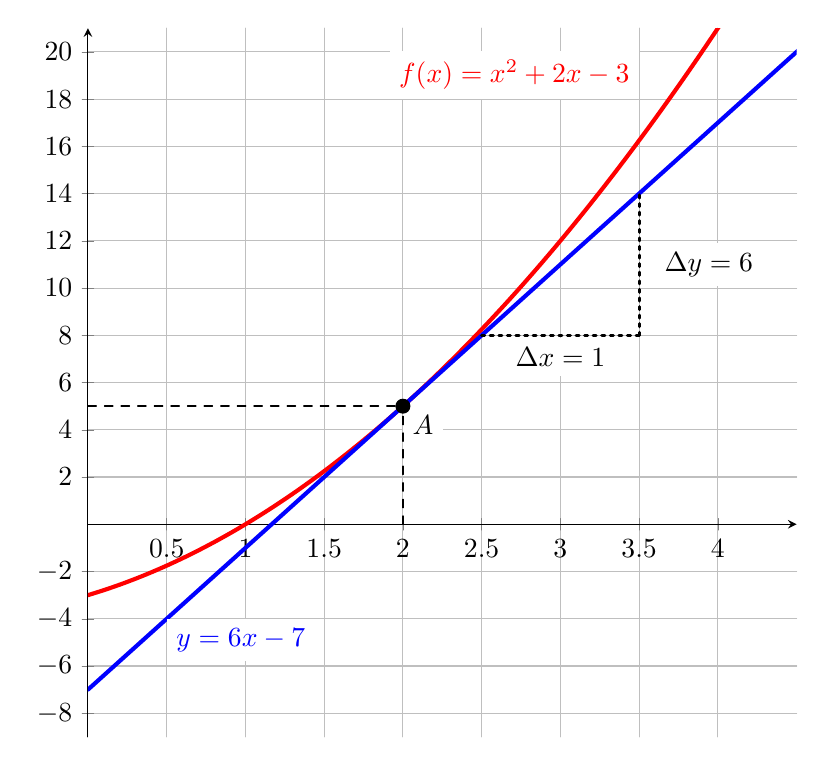
\begin{tikzpicture}[line cap=round,line join=round,>=triangle 45,x=1.0cm,y=1.0cm]
	\begin{axis}[x=2cm,y=0.3cm,axis lines=middle,ymajorgrids=true,xmajorgrids=true,xmin=0,xmax=4.5,ymin=-9,ymax=21,xtick={-1,-.5,...,4},ytick={-8,-6,...,20},]
		\draw[line width=1.5pt,color=red,smooth,samples=50,domain=0.001:5] plot(\x,{(\x)/(1/(\x))+2/(1/(\x))-3});
		\draw[line width=1.5pt,color=blue,smooth,samples=50,domain=0.001:5] plot(\x,{6/(1/(\x))-7});
		\draw [color=black,anchor=north west] (2,5) node[fill=white] {$A$};
		\draw [fill=black] (2,5) circle (2.5pt);
		\draw [color=red,anchor=south east] (3.5,18) node[fill=white] {$f(x)=x^2+2x-3$};
		\draw [color=blue,anchor=north west] (0.5,-4) node[fill=white] {$y=6x-7$};
		\draw [color=black, line width=0.5pt, dashed] (0,5)--(2,5);
		\draw [color=black, line width=0.5pt, dashed] (2,0)--(2,5);
		\draw [color=black, line width=1.1pt, dotted] (2.5,8)--(3.5,8);
		\draw [color=black, line width=1.1pt, dotted] (3.5,8)--(3.5,14);
		\draw [color=black,anchor=west] (3.6,11) node[fill=white] {$\Delta y=6$};
		\draw [color=black,anchor=north] (3,7.9) node[fill=white] {$\Delta x=1$};
	\end{axis}\end{tikzpicture}
\end{document}
